\documentclass[11pt,handout,aspectratio=169]{beamer}


%%%%%%%%% GENERAL PACKAGES
%\usepackage{xcolor}
%\usepackage{pdfpages}
%\usetheme[progressbar=frametitle]{metropolis}
%\setbeamercolor{background canvas}{bg=white}
%\usepackage{appendixnumberbeamer}
%\usepackage{booktabs}
%\usepackage[scale=2]{ccicons}
%\usepackage{pgfplots}
%\usepgfplotslibrary{dateplot}
%\usepackage{xspace}
%\newcommand{\themename}{\textbf{\textsc{metropolis}}\xspace}
%\usepackage[absolute,overlay]{textpos}

%%%%%%%%% COLOR THEME

% Define some colors:
\definecolor{DarkFern}{HTML}{407428}
\definecolor{DarkCharcoal}{HTML}{4D4944}
\definecolor{AlertColor}{RGB}{89,124,158}
\definecolor{HighLight}{RGB}{96,95,134}
\definecolor{Important}{RGB}{234,122,133}
\definecolor{Yellow}{HTML}{00539C}
\colorlet{Fern}{DarkFern!85!white}
\colorlet{Charcoal}{DarkCharcoal!85!white}
\colorlet{LightCharcoal}{Charcoal!50!white}
\colorlet{HighLight2}{AlertColor}
\colorlet{DarkRed}{red!70!black}
\colorlet{DarkBlue}{blue!70!black}
\colorlet{DarkGreen}{green!70!black}
\definecolor{RoyalBlue}{HTML}{00539C}
\definecolor{Peach}{HTML}{EEA47F}
\definecolor{ForestGreen}{HTML}{2C5F2D}
\definecolor{MossGreen}{HTML}{E8FCC9}
% Use the colors:
\setbeamercolor{title}{fg=Fern}
\setbeamercolor{frametitle}{fg=MossGreen,bg=ForestGreen}
\setbeamercolor{normal text}{fg=Charcoal!70!black}
\setbeamercolor{block title}{fg=black,bg=Fern!25!white}
\setbeamercolor{block body}{fg=black,bg=Fern!10!white}
\setbeamercolor{block title alerted}{fg=black,bg=DarkRed!25!white}
\setbeamercolor{block body alerted}{fg=black,bg=DarkRed!10!white}
\setbeamercolor{alerted text}{fg=DarkRed}
\setbeamercolor{itemize item}{fg=Charcoal}



%%%%%%%%% OTHER COMMANDS
\newcommand{\indep}{\perp\!\!\! \perp}
\newcommand{\comment}[1]{}
\newcommand{\bs}{\boldsymbol}
\newcommand{\tr}{\text{trace}}
\newcommand{\sgn}{{\rm sgn}}
\def\T{\top}
%\newcommand{\det}{\text{det}}
\newcommand{\var}{\mathrm{var}}
\newcommand{\cC}{{\cal C}}
\newcommand{\cG}{{\cal G}}
\newcommand{\cV}{{\cal V}}
\newcommand{\cE}{{\cal E}}
\newcommand{\cM}{{\cal M}}
\newcommand{\cP}{{\cal P}}
\newcommand{\cX}{{\cal X}}
\newcommand{\cY}{{\cal Y}}
\newcommand{\X}{\mathbf{X}}
\newcommand{\Y}{\mathbf{Y}}
\newcommand{\x}{\mathbf{x}}
\newcommand{\y}{\mathbf{y}}
\newcommand{\z}{\mathbf{z}}

\newcommand{\argmin}{\operatornamewithlimits{argmin}}
\newcommand{\eps}{\varepsilon}
\newcommand{\<}{\langle}
\renewcommand{\>}{\rangle}


\setbeamertemplate{itemize subitem}{\tiny\raise1.5pt\hbox{\donotcoloroutermaths$\blacktriangleright$}}
\setbeamertemplate{itemize subsubitem}{\tiny\raise1.5pt\hbox{\donotcoloroutermaths$\blacktriangleright$}}
\setbeamertemplate{enumerate item}{\insertenumlabel.}
\setbeamertemplate{enumerate subitem}{\insertenumlabel.\insertsubenumlabel}
\setbeamertemplate{enumerate subsubitem}{\insertenumlabel.\insertsubenumlabel.\insertsubsubenumlabel}
\setbeamertemplate{enumerate mini template}{\insertenumlabel}

\newcommand{\TODO}[1]{{\color{red}{[TODO: #1]}}}


\newcommand{\R}{\mathbb R}
\newcommand{\E}{\mathbb E}
\renewcommand{\P}{\mathbb P}


\DeclareMathOperator*{\cov}{cov}


\newsavebox{\zerobox}
\newenvironment{nospace}
{\par\edef\theprevdepth{\the\prevdepth}\nointerlineskip
  \setbox\zerobox=\vtop to 0pt\bgroup
  \hrule height0pt\kern\dimexpr\baselineskip-\topskip\relax
}
{\par\vss\egroup\ht\zerobox=0pt \wd\zerobox=0pt \dp\zerobox=0pt
  \box\zerobox}

\usepackage{soul}
\makeatletter
\let\HL\hl
\renewcommand\hl{%
  \let\set@color\beamerorig@set@color
  \let\reset@color\beamerorig@reset@color
  \HL}
  \makeatother


\title[STA437-Week1]{STA 437/2005: \\ Methods for Multivariate Data}
\subtitle[]{Week 4: Principal Component Analysis}
\author[Prob Learning]{Piotr Zwiernik}
\institute[UofT]{University of Toronto}
\date{}


\usepackage{Sweave}
\begin{document}

\maketitle

%\begin{frame}{Table of contents}
%  \setbeamertemplate{section in toc}[sections numbered]
%  \tableofcontents%[hideallsubsections]
%\end{frame}



\section{PCA teaser}
% \begin{frame}
% {The Team I}



\begin{frame}[fragile]{Example 1: Decathlon}
The columns are a subset of gene expression measurements, they correspond to 156 genes that show differential expression between cell types:
\scriptsize
\begin{Schunk}
\begin{Sinput}
> data("olympic", package = "ade4")
> athletes = setNames(olympic$tab, 
+   c("m100", "long", "weight", "high", "m400", "m110", "disc", "pole", "javel", "m1500"))
> head(athletes)
\end{Sinput}
\begin{Soutput}
   m100 long weight high  m400  m110  disc pole javel  m1500
1 11.25 7.43  15.48 2.27 48.90 15.13 49.28  4.7 61.32 268.95
2 10.87 7.45  14.97 1.97 47.71 14.46 44.36  5.1 61.76 273.02
3 11.18 7.44  14.20 1.97 48.29 14.81 43.66  5.2 64.16 263.20
4 10.62 7.38  15.02 2.03 49.06 14.72 44.80  4.9 64.04 285.11
5 11.02 7.43  12.92 1.97 47.44 14.40 41.20  5.2 57.46 256.64
6 10.83 7.72  13.58 2.12 48.34 14.18 43.06  4.9 52.18 274.07
\end{Soutput}
\end{Schunk}
\end{frame}


\begin{frame}[fragile]{PCA Biplot for Decathlon data}
PCA Biplot of Olympic Athletes	{\scriptsize
\begin{center}
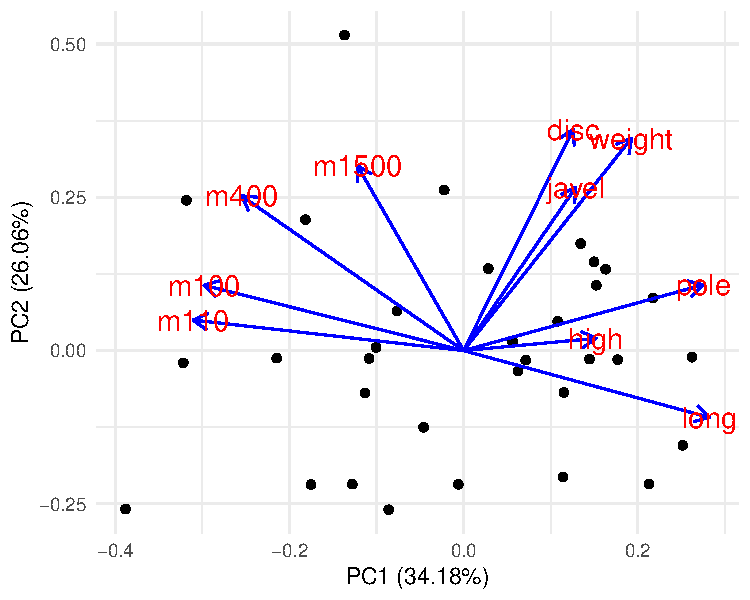
\includegraphics[width=.6\textwidth]{pics/plot4.1.pdf}		
\end{center}}
\end{frame}



\begin{frame}[fragile]{Example 3: Pottery}
Chemical analysis data on Romano-British pottery made in three different regions (kiln 1, kilns 2-3, and kilns 4-5):{\scriptsize
\begin{Schunk}
\begin{Sinput}
> data("pottery", package = "HSAUR2")
> head(pottery)
\end{Sinput}
\begin{Soutput}
  Al2O3 Fe2O3  MgO  CaO Na2O  K2O TiO2   MnO   BaO kiln
1  18.8  9.52 2.00 0.79 0.40 3.20 1.01 0.077 0.015    1
2  16.9  7.33 1.65 0.84 0.40 3.05 0.99 0.067 0.018    1
3  18.2  7.64 1.82 0.77 0.40 3.07 0.98 0.087 0.014    1
4  16.9  7.29 1.56 0.76 0.40 3.05 1.00 0.063 0.019    1
5  17.8  7.24 1.83 0.92 0.43 3.12 0.93 0.061 0.019    1
6  18.8  7.45 2.06 0.87 0.25 3.26 0.98 0.072 0.017    1
\end{Soutput}
\end{Schunk}
}
Question: Do the chemical profiles of each pot suggest different types of pots and if any such types are related to kiln or region.
\end{frame}


\begin{frame}[fragile]{PCA Biplot for Pottery data}
PCA Biplot of Olympic Athletes	{\scriptsize
\begin{center}
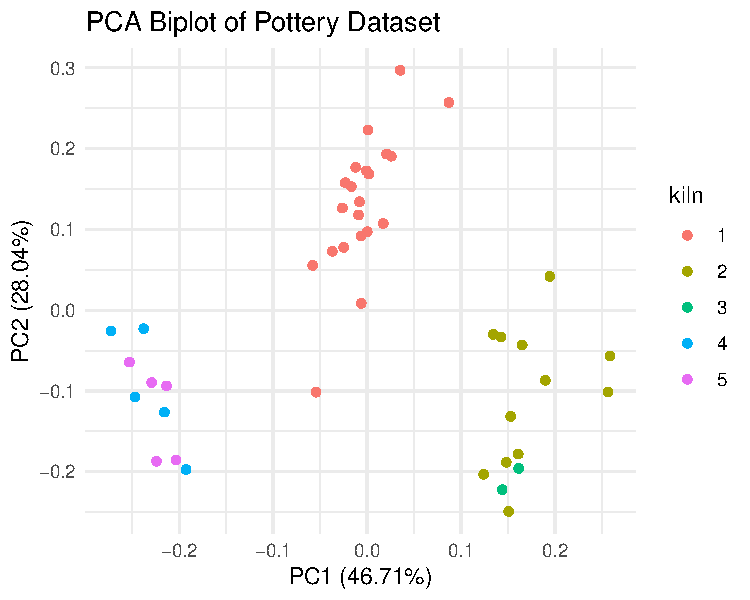
\includegraphics[width=.6\textwidth]{pics/plot4.2.pdf}		
\end{center}}
\end{frame}




\end{document}
